\documentclass[11pt,aspectratio=169,hyperref={colorlinks}]{beamer}
\usetheme{Singapore}
\usecolortheme[snowy, cautious]{owl}

\usepackage[utf8]{inputenc}
\usepackage[T1]{fontenc}
\usepackage[american]{babel}
\usepackage{graphicx}
\usepackage{hyperref}
\hypersetup{
    colorlinks=true,
    urlcolor=[rgb]{0,0,0.61},
    linkcolor=[rgb]{0,0,0.61}}
\usepackage[natbib=true,style=numeric,backend=bibtex,useprefix=true]{biblatex}

%\usepackage{blindtext}

%----------------------------------------------------------------------------------
\definecolor{OwlGreen}{RGB}{51,0,102} 
%----------------------------------------------------------------------------------

\setbeamertemplate{bibliography item}{}
\setbeamerfont{caption}{size=\footnotesize}
\setbeamertemplate{frametitle continuation}{}
\setcounter{tocdepth}{1}
\renewcommand*{\bibfont}{\scriptsize}
\addbibresource{lecture_3.bib}

\usenavigationsymbolstemplate{}
\setbeamertemplate{footline}{%
    \raisebox{5pt}{\makebox{\hfill\makebox[20pt]{\color{gray}
          \scriptsize\insertframenumber}}}\hspace*{5pt}}

\renewcommand*{\thefootnote}{\fnsymbol{footnote}}

%------------------------------------------------------------------------------------------

\author{Patrick Hall}
\title{Responsible Machine Learning\footnote{\tiny{This material is shared under a \href{https://creativecommons.org/licenses/by/4.0/deed.ast}{CC By 4.0 license} which allows for editing and redistribution, even for commercial purposes. However, any derivative work should attribute the author.}}}
\subtitle{Lecture 3:  Fairness}
\institute{The George Washington University}
\date{\today}


\begin{document}
	
	\maketitle
	
	\begin{frame}
	
		\frametitle{Contents}
		
		\tableofcontents{}
		
	\end{frame}


%-------------------------------------------------------------------------------
	\section{Introduction}
%-------------------------------------------------------------------------------

		\subsection*{}

		\begin{frame}
		
			\frametitle{A Responsible Machine Learning Workflow\footnote{\href{https://www.mdpi.com/2078-2489/11/3/137/htm}{\textit{A Responsible Machine Learning Workflow}}}}
			
			\begin{figure}[htb]
				\begin{center}
					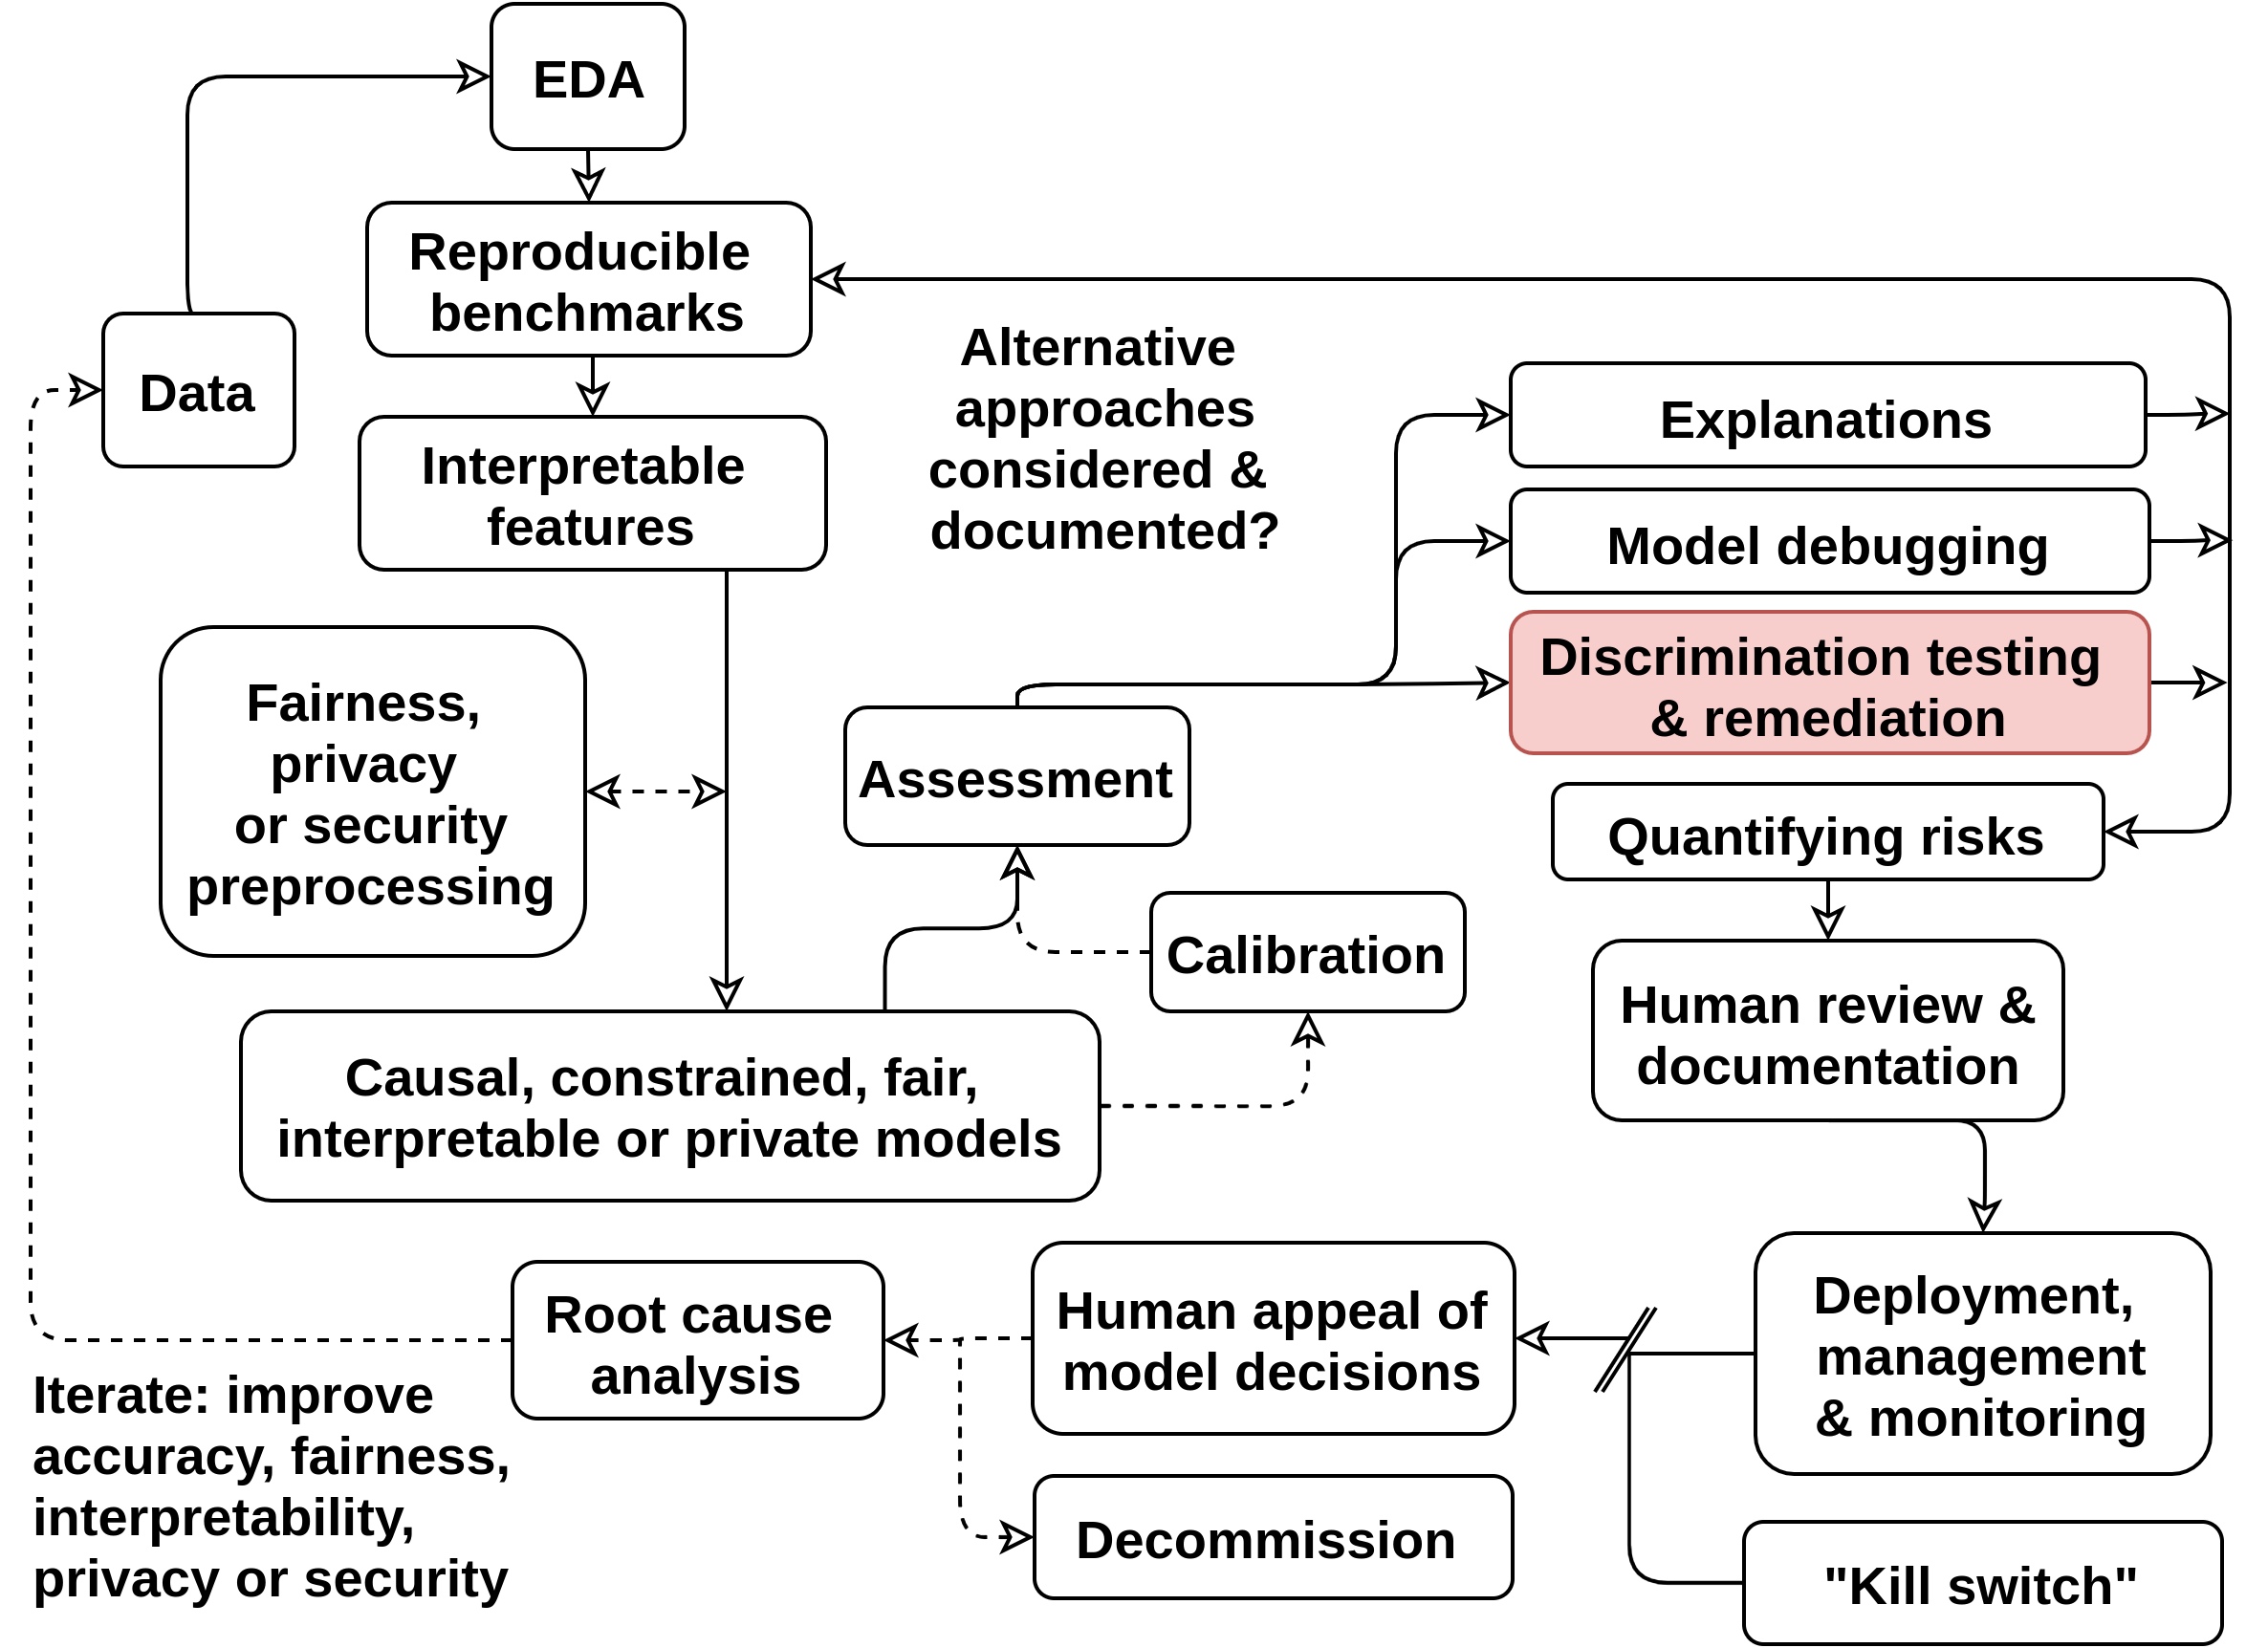
\includegraphics[height=150pt]{../img/rml_diagram_lec3_hilite.png}
					\label{fig:blueprint}
				\end{center}
			\end{figure}		
					
		\end{frame}	


		\begin{frame}				
		
			\frametitle{Why Care About Discrimination in ML?}
			
			\begin{itemize}
				\Large
				\item \textbf{Reputational risk}: 
					\begin{itemize}
						\Large
						\item{\normalsize{Upon encountering a perceived unethical ML system, 34\% of consumers are likely to, ``stop interacting with the company.''\footnote{\scriptsize{See: \href{https://www.capgemini.com/research/why-addressing-ethical-questions-in-ai-will-benefit-organizations/}{Why addressing ethical questions in AI will benefit organizations}.}}}}
					\end{itemize}
				\item Non-compliance fines and litigation costs.
				\item Responsible practice of ML. 
			\end{itemize}
			
		\end{frame}


		\begin{frame}
		
			\frametitle{Elements of Responsible Practice of ML}
		
		  	\begin{figure}[htb]
    				\begin{center}
      					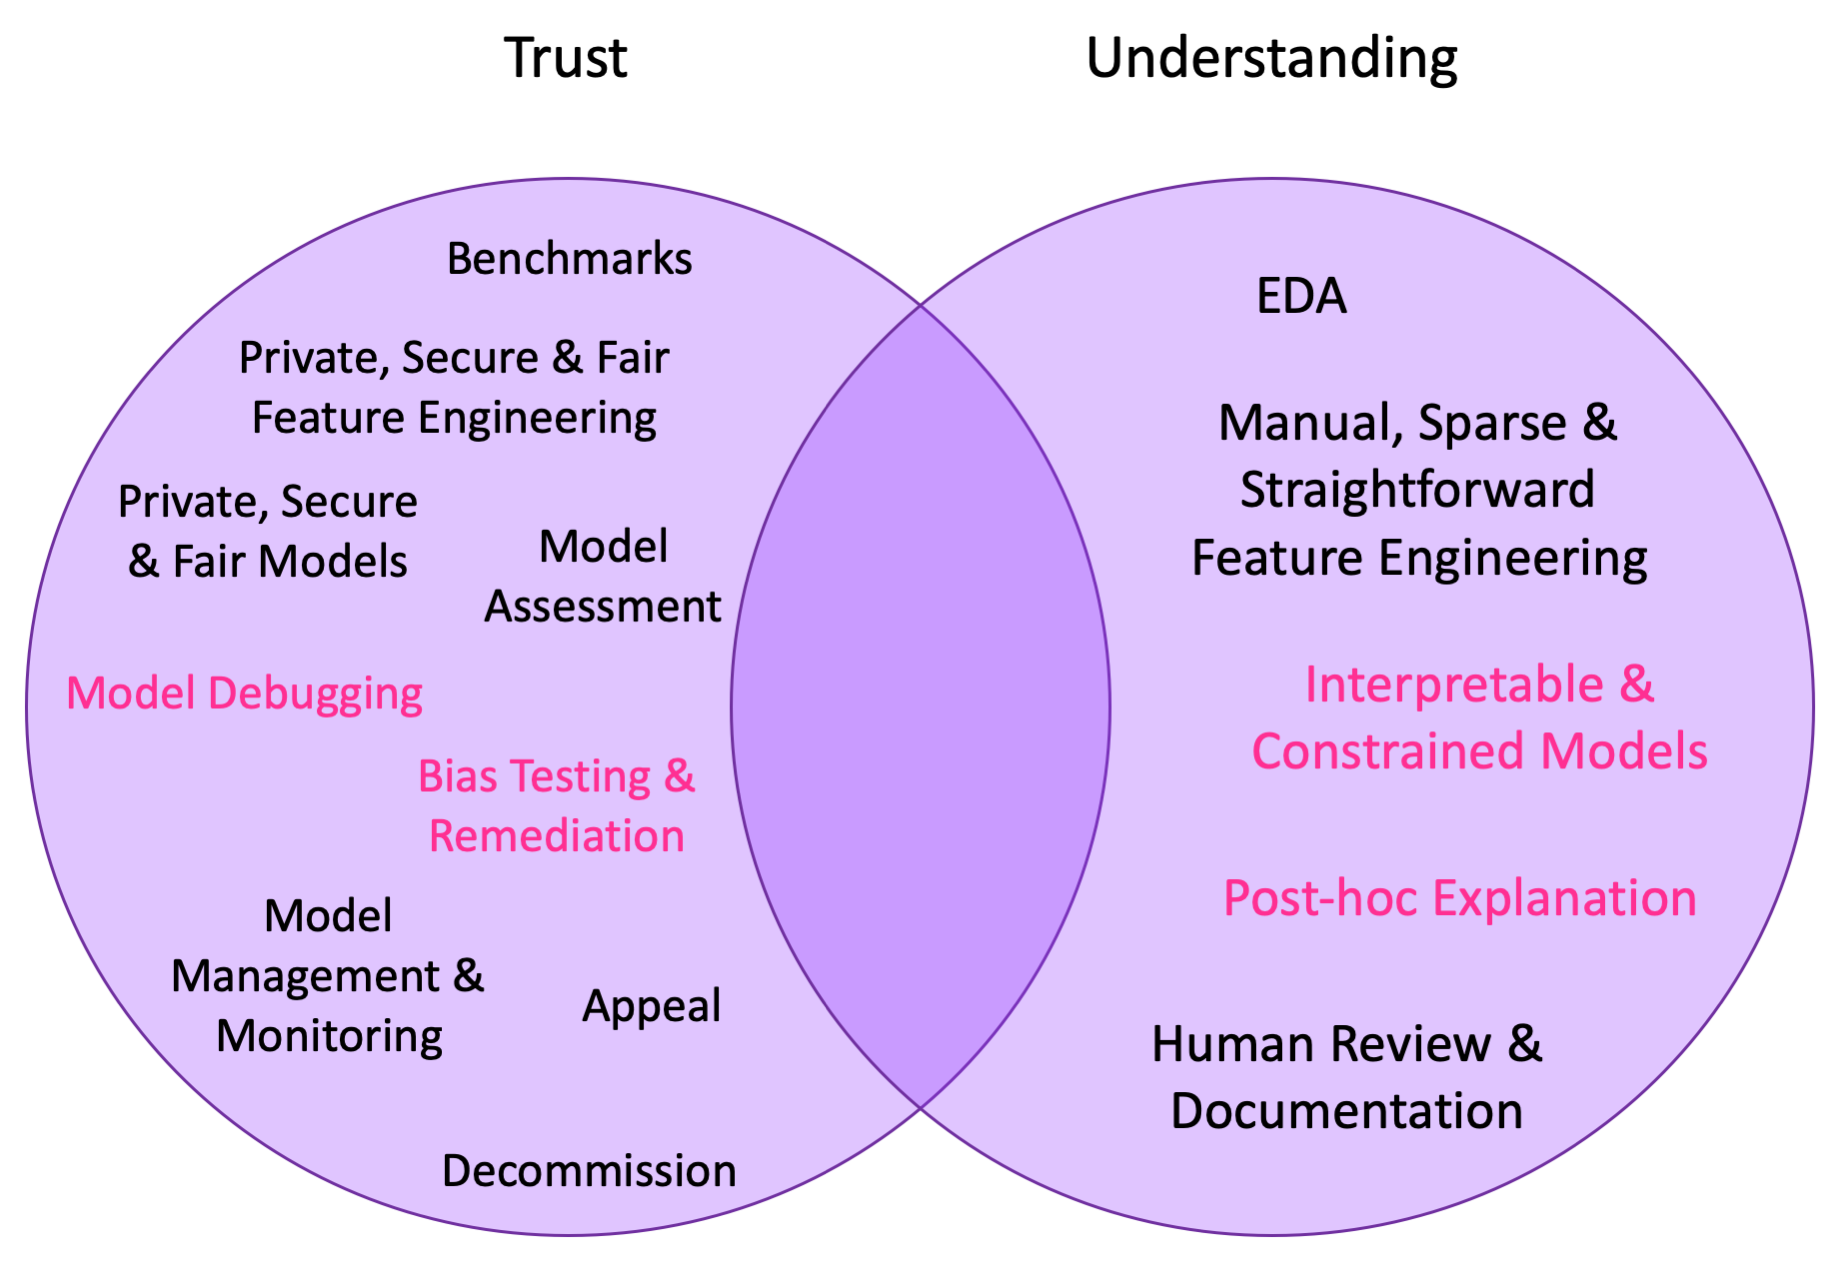
\includegraphics[height=180pt]{../img/trust_understanding.png}
    				\end{center}
  			\end{figure}
		
		\end{frame}

%-------------------------------------------------------------------------------
	\section{Discrimination \& Bias}
%-------------------------------------------------------------------------------
	
		\subsection*{}
	
		\begin{frame}
		
			\frametitle{What Is Bias?}			
					
			\begin{itemize}
			\Large
			\item Almost all data, statistical models, and machine learning (ML) models encode different types of \textit{bias}, i.e., systematic misrepresentations of reality.\\
			\item Sometimes, bias is helpful.
				\begin{itemize}
					\Large
					\item{shrunken and robust $\beta_j$ coefficients in penalized linear models}				\end{itemize}
			\item Other types of bias might be unwanted, unhelpful, or illegal discrimination. 
			\end{itemize}
					
		\end{frame}					
		
		\subsection*{}
		
		\begin{frame}[allowframebreaks]{Title}				
		
			\frametitle{What is Discrimination in ML?}
						
			\noindent In some applications\footnote{\small{e.g., Under the Equal Credit Opportunity Act (ECOA), as implemented by Regulation B, and the Fair Credit Reporting Act (FCRA})}, model predictions should \textbf{\textit{ideally}} be independent of demographic group membership.\\
			\vspace{5pt}
			\noindent In these applications, a model exhibits discrimination if:
			\begin{enumerate}
				\item Demographic group membership is not independent of the likelihood of receiving a favorable or accurate model prediction.
				\item Membership in a \textit{subset} of a demographic group is not independent of the likelihood of receiving a favorable or accurate model prediction (i.e., \textit{local bias}).\cite{hall2019guidelines}
			\end{enumerate}
		\end{frame}
		
		\begin{frame}
		
			\frametitle{What is Discrimination in ML?}	
			
			\noindent \Large Several forms of discrimination may manifest in ML, including:
			\begin{itemize}
				\item Overt discrimination, i.e. \textit{disparate treatment}.
				\item Unintentional discrimination, i.e. \textit{disparate impact} (DI).
				\item Discrimination in ML may or may not be illegal, depending on how it arises and applicable discrimination laws.\cite{hall2019guidelines}
			\end{itemize}
		\end{frame}		
		
		\begin{frame}				
		
			\frametitle{What is Discrimination in ML?}
			
			\noindent Discrimination originates from training data:\\
			\begin{itemize}
				\item Incomplete or inaccurate data, particularly under-representation of minorities, e.g. \href{http://gendershades.org/}{Gender Shades}\cite{gender_shades}.
				\item Accurate but differing patterns of causation, correlation, or dependency between demographic groups and past outcomes, e.g. traditional FICO credit scores.\footnote{\scriptsize{See: \href{https://www.youtube.com/watch?v=rToFuhI6Nlw}{Responsible Data Science: Identifying and Fixing Biased AI}.}}
				\item Explicit encoding of historical social biases into training data, e.g. criminal records.\textsuperscript{$\mathparagraph$}
			\end{itemize}

		\end{frame}

		\begin{frame}				
		
			\frametitle{What is Discrimination in ML?}
			
			ML models can perpetuate or exacerbate discrimination.\\
			\vspace{10pt}
			\noindent \textbf{Group disparities}, i.e. different or inaccurate treatment of entire demographic groups:\\
			\begin{itemize}
				\item Learning different correlations between demographic groups and favorable model outcomes, i.e. \textit{adverse impact}.
				\item Exhibiting different accuracies across demographic groups, i.e. \textit{differential validity}.\textsuperscript{$\mathparagraph$}
			\end{itemize}
			\vspace{5pt}
			\noindent \textbf{Locally}, i.e. different or inaccurate treatment of similar individuals:\\
			\begin{itemize}
				\item Local response function or decision boundary form. 
				\item Capacity to form local complex or latent demographic proxies.
			\end{itemize}
							
		\end{frame}
		
		\begin{frame}				
		
			\frametitle{Common Metrics of Discrimination in ML}
			
			Common metrics of \textbf{\textit{group}} disparities:\\
			\begin{itemize}
				\item Accuracy disparity: $\frac{\text{accuracy}_p}{\text{accuracy}_r}$
				\item Adverse impact ratio: $\frac{\text{\% accepted}_p }{ \text{\% accepted}_r}$ 
				\item Marginal effect: $\text{\% accepted}_p - \text{\% accepted}_r$
				\item Standardized mean difference: $\frac{\bar{\hat{y}}_p - \bar{\hat{y}}_r}{\sigma_{\hat{y}}}$
			\end{itemize}
			\noindent 
			\scriptsize where, $p \equiv \text{protected group}$ and $r \equiv \text{reference group}$ (often white males),\\
			\vspace{5pt}
			$\text{\% accepted}_\text{group} = 100 \cdot \frac{\text{tn}_\text{group}~+~\text{fn}_\text{group}}{N_\text{group}}$, and $\text{accuracy}_\text{group} = \frac{\text{tp}_\text{group}~+~\text{tn}_\text{group}}{N_\text{group}}$.\textsuperscript{$\mathparagraph$}\\
			\vspace{10pt}
			\normalsize
			\textbf{\textit{Local bias}} is much trickier to measure and often an unmitigated risk for consumer-facing ML systems.
		\end{frame}		

%-------------------------------------------------------------------------------
	\section{Remediation}
%-------------------------------------------------------------------------------
	
		\subsection*{}

		\begin{frame}			
		
			\frametitle{How to Fix Discrimination in ML?}
			\Large \noindent 
			\textbf{Fix the process}: ensure diversity of experience in design, training, and review of ML systems.\\
			\noindent 
			\textbf{Fix the data}:
			\begin{itemize}
				\item Collect demographically representative training data.
				\item Select features judiciously, e.g. using \texttt{time\_on\_file} as an input variable as opposed to \texttt{bankruptcy\_flag}.\textsuperscript{$\mathparagraph$}
				\item Sample and reweigh training data to minimize discrimination.\cite{kamiran2012data}
			\end{itemize}
			
		\end{frame}	
		
			
		\begin{frame}			
		
			\frametitle{How to Fix Discrimination in ML?}			
			
			\noindent 
			\textbf{Fix the model}:
			\begin{itemize}
				\item Consider fairness metrics when selecting hyperparameters and cutoff thresholds.
				\item Train fair models directly:
				\begin{itemize}
					\item Learning fair representations (LFR) and adversarial de-biasing.\cite{zemel2013learning}, \cite{zhang2018mitigating}
					\item Use dual objective functions that consider both accuracy and fairness metrics.
				\end{itemize}
				\item Edit model mechanisms to ensure less biased predictions, e.g. with \href{https://github.com/interpretml/interpret}{GA2M} models.
			\end{itemize}		
			\noindent \textbf{Fix the predictions}: 
			\begin{itemize}
				\item Balance model predictions, e.g. reject-option classification.\cite{kamiran2012decision}	
				\item Correct or override predictions with model assertions or appeal mechansims.\cite{hall2019guidelines}, \cite{kangdebugging}
			\end{itemize}
			
		\end{frame}
		
		\subsection*{}
		
		\begin{frame}
		
			\frametitle{How to Fix Discrimination in ML?}		
			\centering
			As part of a responsible ML workflow.\\
			\vspace{10pt}
			{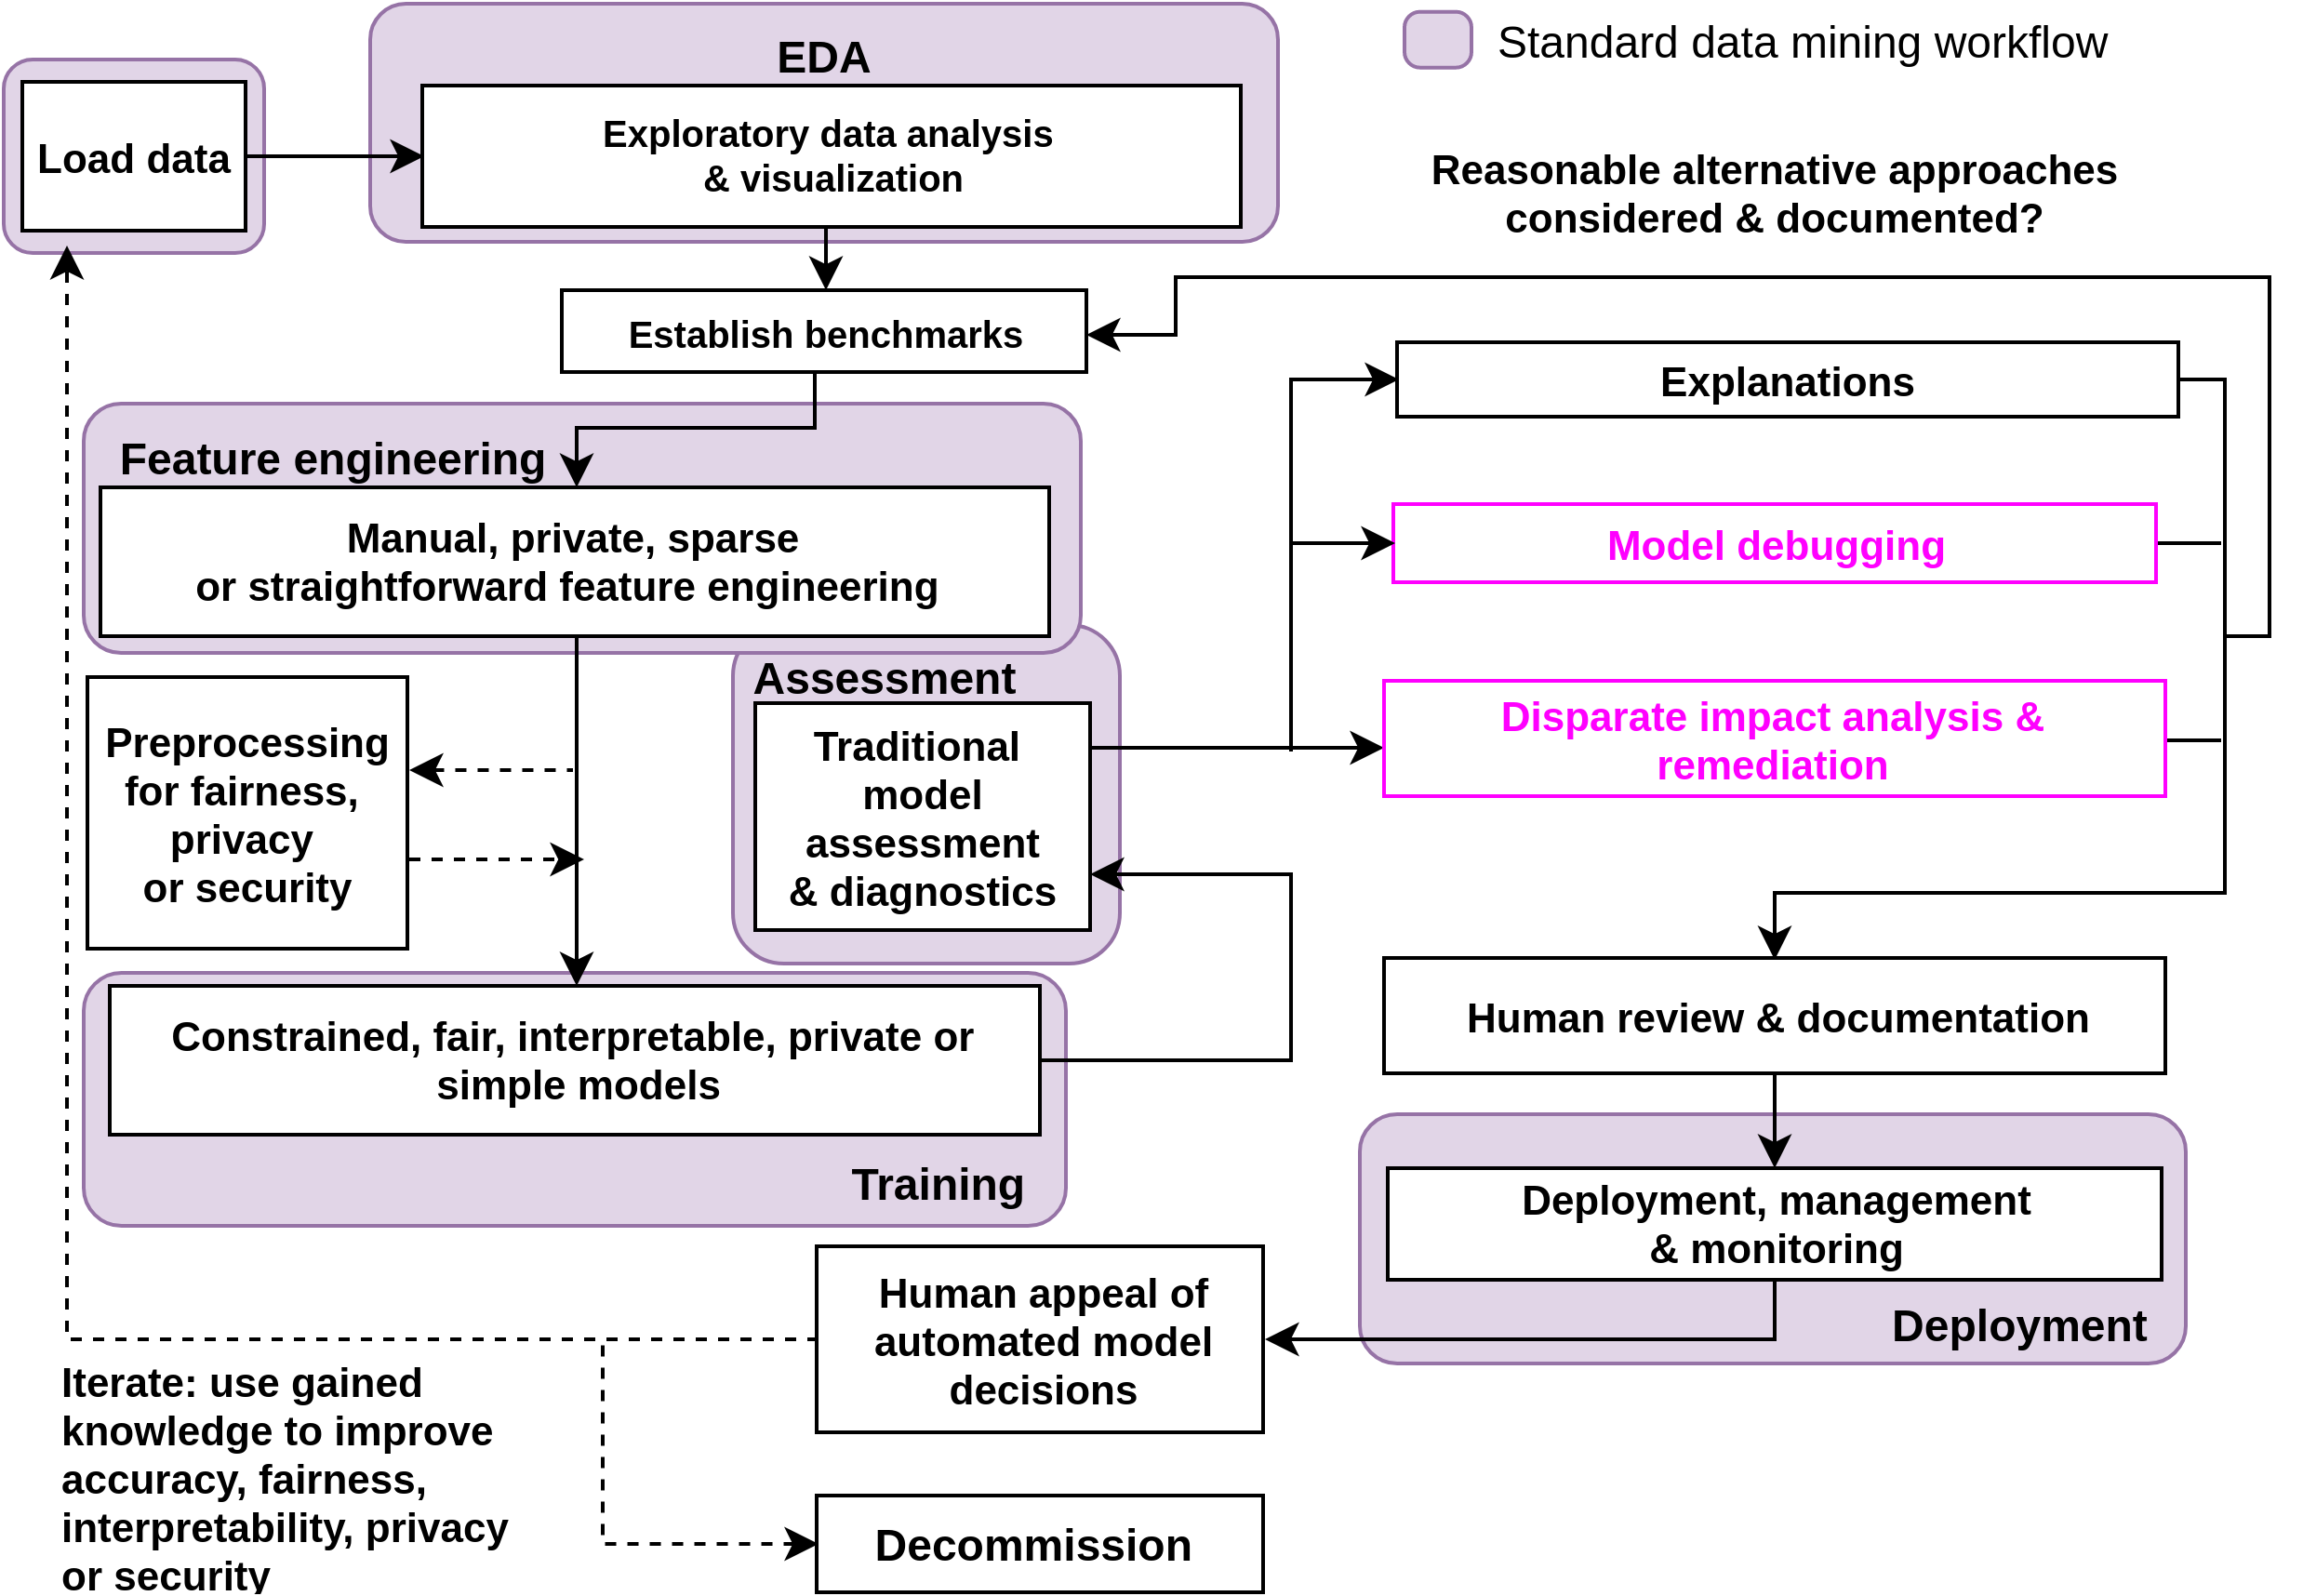
\includegraphics[scale=0.08]{../img/blueprint.png}}
			
		\end{frame}		
		
%-------------------------------------------------------------------------------
	\section{Acknowledgements}
%-------------------------------------------------------------------------------

	\subsection*{}
	
	\begin{frame}
	
		\frametitle{Acknowledgements}
		This presentation borrows heavily from the expertise of Nicholas Schmidt and Bryce Stephens of \href{https://www.bldsllc.com/}{BLDS, LLC}, a leading fair lending compliance firm.
		
	\end{frame}	
	
%-------------------------------------------------------------------------------
%	References
%-------------------------------------------------------------------------------

	\begin{frame}[t, allowframebreaks]
	
		\frametitle{References}
		\printbibliography
		
	\end{frame}

\end{document}